\subsection{Design}
\label{adinjection:sec:design}

In this section, we describe an in-browser approach for identifying third-party
content modifications in web browsers. The approach adds \emph{fine-grained
provenance tracking} to the browser, at the level of individual DOM elements.
Provenance information is used in two ways:
\begin{inparaenum}[\itshape i)\upshape]
    \item to distinguish between content that originates from the web page
    publisher and content injected by an unassociated third party, and
    \item to indicate \emph{which} third party (e.g., extension) is responsible
    for content modifications using provenance indicators.
\end{inparaenum}
By integrating the approach directly into the browser, we guarantee the
trustworthiness of both the provenance information and the visual indicators.
While we consider malicious or exploited browser plug-ins such as Flash Player
outside our threat model, we note that modern browsers take great pains to
isolate plug-ins in least privilege protection domains.

\subsubsection{Content Provenance}
\label{adinjection:sec:design:provenance}

\begin{figure}[t]
    \centering
    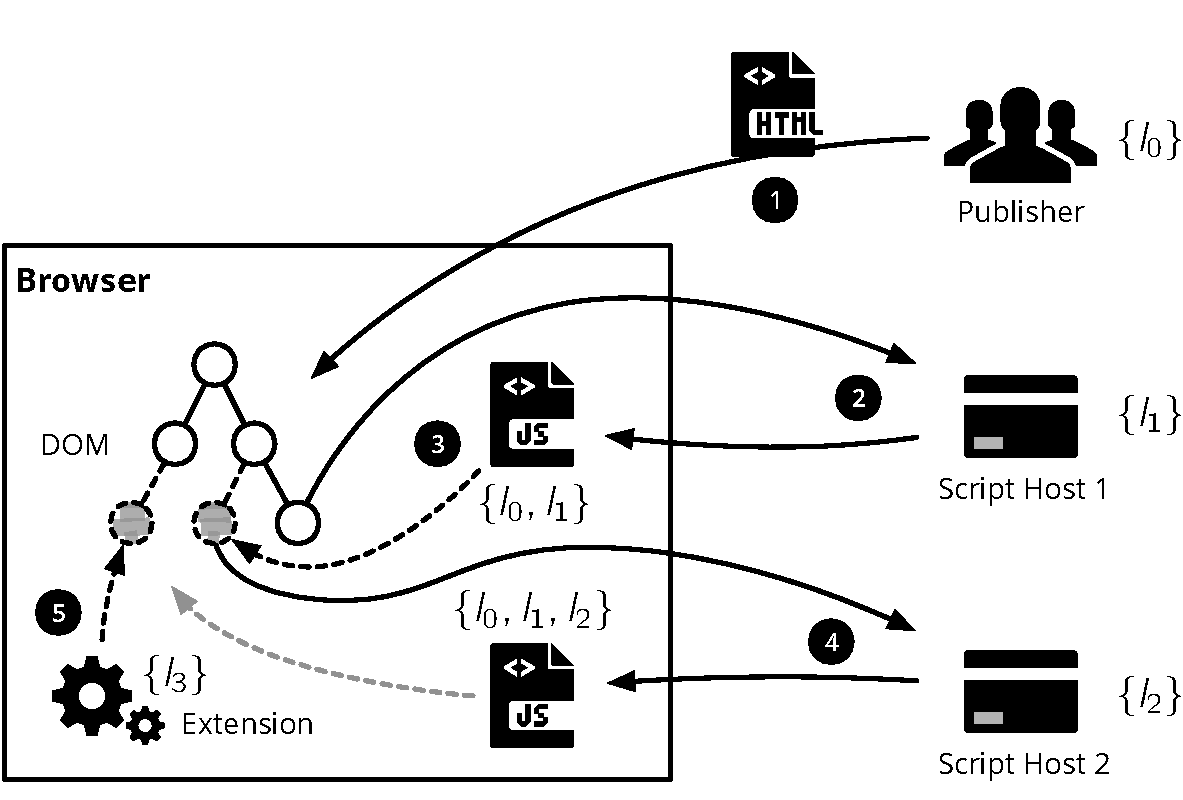
\includegraphics[width=0.7\textwidth]{adinjection/figures/provenance.pdf}
    \caption{Element-granularity provenance tracking.
        \textbf{(1)}~Content loaded directly from the publisher is labeled
        with the publisher's origin, \(l_0\).
        \textbf{(2)}~An external script reference to origin \(l_1\) is performed.
        \textbf{(3)}~DOM modifications from \(l_1\)'s script are labeled with
        the label set \(\left\{l_0,l_1\right\}\).
        \textbf{(4)}~Further external script loads and subsequent DOM
        modifications induce updated label sets -- e.g.,
        \(\left\{l_0,l_1,l_2\right\}\).
        \textbf{(5)}~A DOM modification that originates from an extension
        produces provenance label sets \(\left\{l_0, l_1, l_2, l_3\right\}\) for
        the element.}
    \label{adinjection:fig:provenance}
\end{figure}


Web pages are composed of HTML that references resources such as stylesheets,
scripts, images, plug-ins such as Flash objects, or even other web pages loaded
inside frames. The document object model (DOM) is a natural structural
representation of a web page that can be manipulated through a standard API, and
serves as a suitable basis for provenance tracking. In particular, our system
tracks the provenance of each element \(e\) contained in a DOM. Provenance for a
DOM element is recorded as a set of labels \(\ell \in
\mathcal{P}\left(L\right)\), where the set of all labels \(L\) corresponds to a
generalization of standard web origins to include extensions. That is, instead
of the classic origin 3-tuple of \(\left\langle \texttt{scheme}, \texttt{host},
\texttt{port} \right\rangle\), we record

\begin{align*}
L &= \left\langle S, I, P, X \right\rangle \\
S &= \left\{ \texttt{scheme} \right\} \cup \left\{ \texttt{``extension''} \right\} \\
I &= \left\{ \texttt{host} \right\} \cup \left\{ \texttt{extension-identifier} \right\} \\
P &= \left\{ \texttt{port} \right\} \cup \left\{ \texttt{null} \right\} \\
X &= \left\{0, 1, 2, \ldots\right\}
\end{align*}

In other words, a label is a 4-tuple that consists of a normal network scheme or
\texttt{extension}, a network host or a unique extension identifier, a port or
the special \texttt{null} value, and an index used to impose a global total
order on labels as described below. While browsers use different extension
identifiers, including randomly-generated identifiers, the exact representation
used is unimportant so long as there is a one-to-one mapping between extensions
and identifiers and their use is locally consistent within the browser. An
overview of provenance tracking is depicted in
Figure~\ref{adinjection:fig:provenance}.

\paragraph{Static Publisher Provenance}

Content provenance tracking begins with a web page load. As the DOM is parsed by
the browser, each element is labeled with a singleton label set containing the
origin of the publisher, \(\left\{l_0\right\}\). Thus, static provenance
tracking is straightforward and equivalent to the standard use of origins as a
browser security context.

\paragraph{Dynamic Publisher Provenance}

Content provenance becomes more interesting in the presence of dynamic code
execution. As JavaScript can add, modify, and remove DOM elements in an
arbitrary fashion using the DOM API exposed by the browser, it is necessary to
track these modifications in terms of provenance labels.

New provenance labels are created from the publisher's label set
\(\left\{l_0\right\}\) as follows. Whenever an external script is referenced
from the initial DOM resulting from the page load, a new label \(l_i, i \in
\left\{1,2,\ldots\right\}\) is generated from the origin of the script. All
subsequent DOM modifications that occur as a result of an external script loaded
from the initial DOM are recorded as \(\left\{l_0,l_i\right\}\). Successive
external script loads follow the expected inductive label generation process --
i.e., three successive external script loads from unique origins will result in
a label set \(\left\{l_0,l_i,l_j,l_k\right\}\). Finally, label sets contain
unique elements such that consecutive external script loads from a previously
accessed origin are not reflected in the label for subsequent DOM modifications.
For instance, if the web page publisher loads a script from the publisher's
origin, then any resulting DOM modifications will have a provenance label set of
\(\left\{l_0\right\}\) instead of \(\left\{l_0,l_0\right\}\). Content provenance
is propagated for three generic classes of DOM operations: element insertion,
modification, and deletion.

Element insertions produce an updated DOM that contains the new element labeled
with the current label set, and potentially generates a new label set if the
injected element is a script. Element modifications produce a DOM where the
modified element's label set is merged with the current label set. Finally,
element deletions simply remove the element from the DOM.

\paragraph{Extension Provenance}

The third and final form of provenance tracking concerns content modifications
due to DOM manipulations by extensions. In this case, provenance propagation
follows the semantics for the above case of dynamic publisher provenance. Where
these two cases differ, however, is in the provenance label initialization.
While provenance label sets for content that originates, perhaps indirectly,
from the web page publisher contains the publisher's origin label \(l_0\),
content that originates from an extension is rooted in a label set initialized
with the \emph{extension's} label. In particular, content modifications that
originate from an extension \emph{are not labeled} by the publisher's origin. An
exception to this occurs when the extension, either directly or indirectly,
subsequently loads scripts from the publisher, or modifies an existing element
that originated from the publisher.

\subsubsection{Content Provenance Indicators}
\label{adinjection:sec:design:indicators}

With the fine-grained content provenance scheme described above, identifying the
principal responsible for DOM modifications is straightforward. For each
element, all that is required is to inspect its label set \(\ell\) to check
whether it contains the label of any extension.

A related, but separate, question is how best to relay this information to the
user. We report on the specific design choices we made with respect to
provenance indicators in the presentation of our implementation in
Section~\ref{adinjection:sec:impl}.
